\mychapter{1}{Analýza}

V biznis sektore je neustála potreba monitorovať a kontrolovať firemné procesy. Čím je podniková štruktúra hlbšia, procesy komplexnejšie a narastá počet zamestnancov, tým stúpa náročnosť riadenia a manažmentu podniku. Komplexné projekty sú len zriedkavo vypracované podľa pôvodného časového plánu. Toto meškanie je často spôsobené zlou koordináciou pracovných procesov. Vo firemných  procesoch jednotlivé úlohy za sebou nasledujú v určitom poradí, ktoré musí byť prísne dodržané. Aj meškanie drobnej úlohy dokáže dominovým efektom zastaviť vykonanie nasledovných úloh. V konečnom dôsledku tak malé zaváhanie môže spôsobiť obrovské oneskorenie a finančné straty.   Vzniká tak potreba jasne vymedziť jednotlivé kroky práce a minimalizovať administráciu a možné chyby. Riešenie tohto problému je možné riešiť využitím Workflow management systémov.  WfMS ponúkajú možnosť explicitne zadefinovať firemné procesy, pričom dokážu automaticky zabezpečiť správnosť vykonávania jednotlivých úloh v korektnom poradí. Vo firemnom prostredí tak nastane poriadok a zjednoduší sa administrácia. Hlavnou nevýhodou WfMS sú náklady na samotnú implementáciu. Väčšina WfMS sa vyvíja pre potreby konkrétneho podniku, pričom náklady na ich naprogramovanie presahujú finančnú kapacitu stredných a drobných firiem. Na trhu sa tak objavujú generické WfMS systémy, ktoré dokážu zabezpečiť využívanie procesov viacerými organizáciami súčasne. 

Možným nástrojom na implementovanie WfMS sa naskytuje použitie Petriho sietí. Petriho siete sú jasne formálne a matematicky definované, pričom ich modelovanie je jednoduché a intuitívne. Medzi hlavné výhody môžeme považovať grafické znázornenie, ktoré uľahčuje pochopenie princípov a fungovania tohto modelu. Ak pripojíme fakt, že adaptácia Petriho sietí na WfMS nie je komplikovaná , môžeme tak Petriho siete považovať za vhodný nástroj na modelovanie WfMS. 

Petriho siete sú dobrým nástrojom na modelovanie procesov vo WfMS, nedokážu nám však samy o sebe zabezpečiť riadenie prístupových práv. Pre potreby WfMS systémov je najpoužívanejšia metóda riadenia rolí RBAC. Tento model nám ponúka lepšiu alternatívu k bežne používaným systémom DAC (data access control) a MAC (mandatory access control). Zásadný rozdiel medzi RBAC a ostatnými modelmi spočíva v oddelení prístupových práv od samotných používateľov. To zabezpečuje možnosť namodelovať proces nezávisle od používateľskej časti. Okrem toho má mnoho výhôd, ktoré pramenia z toho, že tento model je zhodný s tým, ktorý je vo firmách prirodzene zaužívaný.



%---------------------------------- začiatok sekcie Workflow management systém ----------------------------------------

\section{Workflow management systém}
V každom podniku je zaužívaná určitá logistika, nastavenie procesov na základe ktorých prebieha celé riadenie a manažment práce. Cieľom workflow manažmentu (WfM) je zaistiť aby bola táto logistika správne vykonávaná, čo znamená určiť kto má v danom momente spustiť akú úlohu. S narastajúcou veľkosťou podniku alebo zložitosťou procesov, manažment riadenia príde do bodu, kedy je len veľmi ťažko ovládateľný. Naskytuje sa tak potreba, aby sa celý manažment zautomatizoval. Vzniká tak workflow management systém (WfMS).Workflow Management Coalition definoval termín WfMS ako systém, ktorý kompletne určí, manažuje a vykonáva workflow cez softvér, ktorý má určené vykonávanie jednotlivých úloh na základe počítačovej reprezentácie workflow logiky. \cite{aalst}\\

%Základom každého WfMS je zabezpečiť  kontrolu a koordináciu nad procesmi, ktoré zahrňujú ľudskú prácu v organizovanom prostredí.  
%pre automatizáciu firemných procesov , v priebehu ktorého informácia putuje z jednej aktivity na ďalšiu, od jedného účastníka k druhému za určitých zadefinovaných pravidiel .
%Dôležitým faktorom pri simulácii daných procesov je zabezpečiť korektné poradie vykonávaných úloh. 


Workflow systémy sú založené na jednotlivých prípadoch (cases). Ako jednotlivý prípad si môžeme predstaviť konkrétnu požiadavku, ako je napríklad založenie si účtu, objednávka, spísanie závete a podobne. Jednotlivé prípady sú často krát spúšťané samotnými zákazníkmi, ale nie je to pravidlo. Hoci takýchto prípadov môže vzniknúť v systéme mnoho, ich priebeh je riadený za pomoci jednotnej workflow logiky. Každý prípad je unikátny a má konečnú životnosť.  Úloha, ktorá sa vykonáva v konkrétnom prípade sa nazýva pracovaná jednotka (working item).
Spôsob vykonávania jednotlivých úloh (pracovných jednotiek) v prípade  je určený prostredníctvom definície workflow procesov. \cite{aalst}  \\	 



Každý prípad vo WfMS má svoj začiatok a koniec. Medzitým sa proces nachádza v určitom stave, ktorý je definovaný prostredníctvom:
\begin{itemize}
	\item architektúry daného prípadu - určuje nám ako sa môže daný prípad vyvíjať. 
	\item doposiaľ splnených podmienok - zistíme tak aktuálnu "polohu", v akej sa daný prípad nachádza 
	\item hodnoty atribútov v danom prípade - atribúty nám definujú isté podmienky. Predstavme si prípad šetrenia peňazí do pokladničky. Do pokladničky budeme vkladať peniaze, dokiaľ suma v pokladničke nepresiahne určitú hodnotu. V našom prípade sú atribútom peniaze
\end{itemize}

\subsection{Úloha}
Úloha je základnou logickou jednotkou workflow systému. Ako taká je nedeliteľná a v systéme sa musí vždy vykonať ako celok. V prípade neúspechu úlohy tak treba úlohu spustiť celú odznova. Je však možné rozlišovať medzi spustením a ukončením úlohy. 

\subsection{Proces}
Proces definuje spôsob, akým sa vykonajú určité úlohy v konkrétnom prípade. Proces môže byť vo viacerých prípadoch rovnaký ale môže sa takisto odlišovať. Tieto odlišnosti v procese môžu byť napríklad spôsobené smerovacími konštrukciami, za pomoci ktorých je prípad namodelovaný. V prípade vybavovanie pôžičky môže byť žiadosť pre Ferka zamietnutá, zatiaľ čo taká istá žiadosť bude pre Janka schválená.

\subsection{Smerovacie konštrukcie}
	Postupnosť vykonávania  úloh v systéme je určená na základe smerovania prípadu. V jednotlivých vetvách určujeme pre každú úlohu smerovacie konštrukcie, čím umožňujeme vytvoriť  pre prípad odlišné životné cykly. Využívame štyri základné: 
\begin{itemize}
	\item sekvenčné - úlohy sa vykonávajú za sebou v poradí,v akom nasledujú
	\item paralelné – úlohy sa vykonávajú paralelne nezávisle na sebe za pomoci AND-splitov a AND-joinov.
	\item podmienené – vykonávanie úloh závisí od definovaných podmienok. Realizácia sa vykonáva za pomoci OR-splitov a OR-joinov
	\item iteračné- vykonanie jednej alebo viacerých úloh viackrát za sebou
\end{itemize}

\begin{figure}[h]
	\centerline{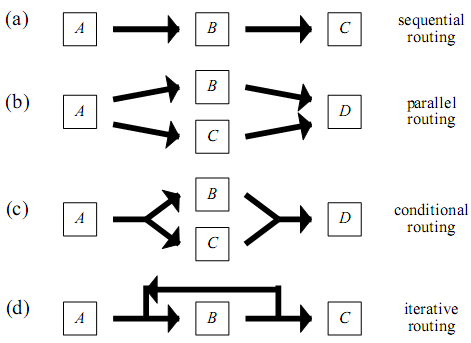
\includegraphics[width=0.6\textwidth]{images/smerovacie_konstrukcie}}
	\caption[smerovacie konštrukcie]{Smerovacie konštrukcie vo workflow systémoch podľa \cite{workflow_systemy}}
	\label{obr:cursus}
\end{figure}

%
\subsection{Výhody použitia WfMS}
Workflow management systém ponúka možnosť oddeliť procesnú časť, čím sa zabezpečia nasledovné výhody:
\begin{itemize}
	\item zabezpečí sa tak jednotná funkcionalita manažmentu a oddelí sa od zvyšku systému. Tradične sa táto funkcionalita rozprestiera v celom systéme. Vďaka tejto separácii je možné rovnakú funkcionalitu použiť na viac ako jednu úlohu.
	\item aplikácie sú nezávislé od manažmentu , čo umožňuje upravovať logiku aj po implementovaní systému
	\item k logickej vrstve je možné pridávať rôzne aplikácie a rozšíriť tak funkcionalitu systému
	\item definovanie a návrh procesu je možné diagnostikovať a vopred tak zabrániť nežiaducim chybám
	\item z pohľadu manažmentu je možné v konkrétnom prípade identifikovať, v akom stave sa prípad nachádza. Celý proces sa tak ľahšie monitoruje. Dá sa zistiť, kto má v danom prípade a čase čo vykonávať. Celé vykonávanie procesu je pod drobnohľadom, čím sa urýchli čas vykonania celého procesu. V prípade problému vo vykonávaní prípadu, je možné rýchlo identifikovať zdroj
	
\end{itemize}

\subsection{Riadenie zrojov vo WfMS}
Pod pojmom zdroj rozumieme jednotku, ktorá je určená na vykonávanie úlohy. Môžme si pod tým predstaviť počítač (server, tlačiareň, fax ... ) alebo človeka ako pracovnú jednotku. V biznis prostredí väčšinu zdrojov tvoria jednotliví pracovníci a zákazníci, nie je to však pravidlo.

Jednotlivé zdroje sa môžu zoskupovať do skupín s podobnou charakteristikou. Ak majú rovnakú funkcionálnu charakteristiku, nazývame túto skupinu rola.
Ako príklad roly si môžeme predstaviť akúkoľvek pracovnú pozíciu a pod samotnými pracovnými zdrojmi samotného zamestnanca. Pridelenie právomocí zdrojom sa udeľuje nepriamo pomocou rol. Týmto spôsobom sa oddelí návrh procesu od jednotlivých používateľov. Taktiež sa tým uľahčí administrácia a zabráni sa deadlockom. Ak by sme totiž priradili úlohu ku konkrétnemu zdroju, nastali by problémy po vymazaní daného zdroja a samotný proces by nebolo možné ukončiť.


%---------------------------------- Koniec sekcie Workflow management systém ----------------------------------------





%----------------------------------Začiatok sekcie Petriho siete----------------------------------------

\section{Petriho siete}
%PETRI, C.A. - REISIG, W. 2008 Petri net. [online] [cit. 27.04.2016]. Dostupné na
%internete: <http://www.scholarpedia.org/article/Petri_net>


%Prof. Dr. Carl Adam Petri [online] [cit. 27.04.2016].
%Dostupné na internete: <http://www.informatik.unihamburg.
%de/TGI/mitarbeiter/profs/petri_eng.html>
\subsection{História}
Petriho siete vymyslel nemecký matematik Carl Adam Petri už ako 13 ročný na modelovanie chemických procesov. Neskôr ich popísal vo svojej dizertačnej práci "Communication with Automata" \cite{petri} v roku 1962. Časom sa však Petriho siete menili a dopĺňali. Dnes už podľa \cite{gabova_kniha} poznáme viacero definícii Petriho sietí. 


\subsection{Všeobecná definícia Petriho siete}
Petriho sieť je podľa 
%\cite{desel} 
 zvláštny typ orientovaného grafu spolu so začiatočným stavom (začiatočným značkovaním) - PN = ( $N, M_{0}$ ). 
Obsahuje dva typy uzlov nazývanými: \emph{place}  (miesto) a \emph{transition} (prechod). Tieto uzly môžu byť spolu prepojené prostredníctvom orientovanej hrany (arc). Spojenie medzi dvoma uzlami rovnakého typu nie je povolené.
\\
\\
Graf Petriho siete obsahuje: 
\begin{itemize}
	\item miesta - označované krúžkom 
	\item prechody - označené obdĺžnikom
	\item hrany - spájajú jednotlivé uzly. Hrany môžu mať určitú násobnosť. Poznáme tieto typy hrán: 
		\begin{itemize}
			\item hrana z miesta do prechodu
			\item hrana z prechodu do miesta
		\end{itemize}
	\item váha hrany - reprezentuje násobnosť hrany
	\item značkovanie - priraďuje každému miestu počet značiek (tokenov) - m-rozmerný vektor nezáporných celých M, M(p)- počet značiek v mieste p 
\end{itemize}

\subsubsection*{Formálna definícia}
Pre formálne opísanie Petriho sietí použijeme definíciu z 
%\cite{}
.\\
	Petriho sieť je orientovaný bipartitný graf reprezentovaný päticou (P,T,F,W,m$_{0}$), kde:\\
\begin{quotation}
	\noindent P = \{$ p_{1}, ... ,p_{n}$ \} - konečná neprázdna množina miest;\\
	T = \{$ t_{1}, ... ,t_{n}$ \} - konečná neprázdna množina prechodov;\\
	{$ P \cap T = \emptyset,P \cup T \neq \emptyset $ }; \\
	{$ F\subseteq ( P x T ) \cup (T x P)$}  - množina hrán (toková relácia);\\
	{$ W : F \rightarrow N \cup \{ 0\}$} - váhová funkcia ;\\
	{$ m_{0} : P \rightarrow N \cup \{ 0\}$} - počiatočné značkovanie;\\
\end{quotation}

\subsection{Pravidlá pre spúšťanie prechodov}
\begin{enumerate}
	\item Prechod je aktivovaný , ak každé z jeho vstupných miest obsahuje aspoň w(p,t) značiek
	\item Spustenie prechodu t spôsobí zrušenie w(p,t) značiek v každom vstupnom mieste p prechodu t a pridanie w(t,p) značiek do každého výstupného miesta p prechodu t;	
\end{enumerate}

\subsection{Príklad}
Na obrázku \ref{obr:voda} môžeme vidieť jednoduchú Petriho sieť ktorá znázorňuje spojenie dvoch prvkov vodíka a kyslíka na vytvorenie vody. Máme tri miesta. Dve z nich nám predstavujú jednotlivé prvky a tretie predstavuje molekulu vody H$_{2} $0. Medzi nimi je prechod ktorý v tejto sieti znázorňuje spojenie dvoch prvkov do jednej molekuly. Medzi miestom O a prechodom máme jednoduchú hranu, zatiaľ čo z miesta H do prechodu máme hranu násobnosti dva. Jednotlivé násobnosti znázorňujú, koľko tokenov (prvkov) treba skonzumovať z každého miesta, aby bolo možné prechod spustiť. Na druhej strane vidíme jednoduchú hranu z prechodu do miesta  H$_{2} $0, ktorá nám značí, že po skonzumovaní značiek z miest O a H sa vytvorí práve jedna značka v mieste H$_{2} $0 (vyprodukuje sa práve jedna molekula ). 

\begin{figure}[h]
	\centerline{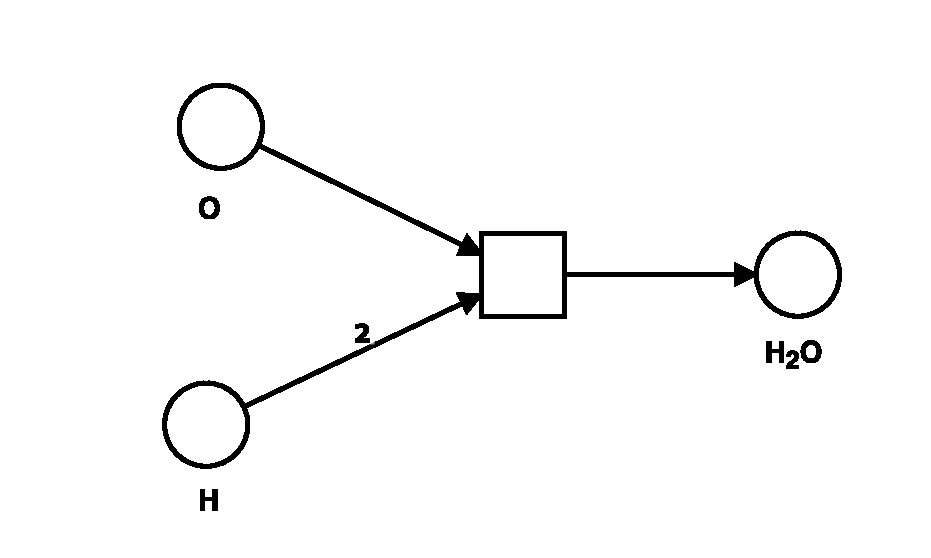
\includegraphics[width=0.4\textwidth]{images/vojvoda}}
	\caption{Petriho sieť na ''vytvorenie'' vody}
	\label{obr:voda}
\end{figure}


Pre spustenie tohto procesu je potrebné aby bola v mieste ''O'' minimálne jedna značka a v mieste ''H'' značiek minimálne dve. Po spustení prechodu sa v miestach vstupujúcich do prechodu odoberie počet tokenov daný násobnostou hrany. Naopak vo výstupnom mieste sa značky podľa násobnosti hrany pridajú pridajú.  

\begin{figure}[h]
	\centerline{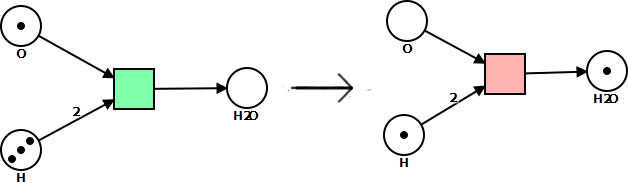
\includegraphics[width=0.9\textwidth]{images/vojvoda2}}
	\caption{Spustenie siete s jedným žetónom v mieste ''O'' a troma žetónmi v mieste ''H''}
	\label{obr:voda2}
\end{figure}





\subsection{Implementovanie Petriho sietí na workflow management systém}
\label{kap:teoria_petriho_siete_na_workflow}
V minulosti sa objavilo niekoľko systémov , ktoré sa snažili implementovať WfMS, ale po čase narazili na problémy, lebo ich architektúra nespĺňala náležité požiadavky. Mnohé z nich nedokázali súčasne implementovať paralelné a alternatívne smerovanie, ostatné narazili na problémy, keď ich aplikácia modelovala WfMS len pomocou udalostí (pri vykonaní úlohy sa systém nedostal do určitého stavu, ale na udalosť nasledovalo okamžité spustenie ďalšej udalosti).
W.M.P. van der Aalst v \cite{workflow_vyhody}
vysvetlil 3 hlavné výhody použitia Petriho sietí na modelovanie workflow management systému:
\begin{itemize}
	\item formálna sémantika spolu s grafickou reprezentáciu
	\item stavové modelovanie namiesto udalostného - toto riešenie umožňuje vidieť stav v akom sa proces nachádza a takisto rozlišuje medzi povolenín a vykonaním úlohy  %(Porovnanie na obr. ----DOPLNIŤ-----)
	\item analýza – vďaka tomu, že sú Petriho siete dobre matematicky popísané, umožňujú dobre analyzovať workflow sieť, čo umožní získať štatistické dáta, prípadne zamedziť problémom
\end{itemize}

Mapovanie WfMS na Petriho siete je možné ľahko ukázať. Úlohy sú mapované na prechody. Závislosti sa mapujú prostredníctvom miest a hrán. Jednotlivé prípady môžu byť odlíšené rôznou farbou tokenov v rozšírených Petriho sieťach. Stav, v akom sa prípad nachádza definuje rozloženie tokenov
Petriho sieť, ktorá modeluje WfMS sa nazýva WorkFlow sieť (WF-sieť). Aby Petriho sieť bola súčasne WF-sieťou, musí spĺnať tieto podmienky
\begin{itemize}
	\item PN má dve špeciálne miesta: miesto ''I'' a miesto ''O'', ktoré reprezentujú počiatočný a koncový stav 
	\item  ak pridáme prechod ''t'' do PN , ktorý spája miesto ''I'' a ''O'', potom je PN silno spojená. To znamená, že pre každý pár uzlov X a Y  existuje priama cesta od X do Y. 
\end{itemize}

\subsubsection{Smerovacie konštrukcie}
\begin{figure}[h]
	\centerline{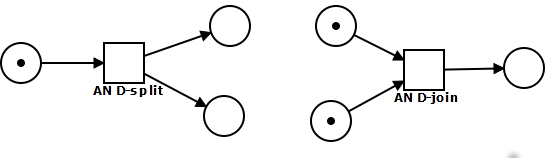
\includegraphics[width=0.7\textwidth]{images/and}}
	\caption[and]{AND konštrukcia v Petriho sieti}
	\label{obr:cursus}
\end{figure}

\begin{figure}[h]
	\centerline{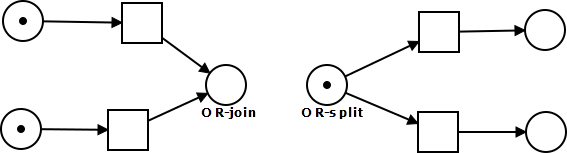
\includegraphics[width=0.7\textwidth]{images/or}}
	\caption[or]{OR konštrukcia v Petriho sieti}
	\label{obr:cursus}
\end{figure}

\begin{figure}[h]
	\centerline{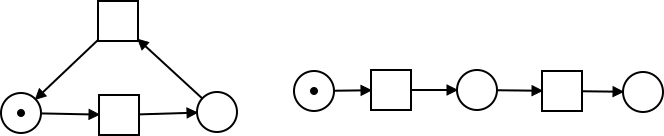
\includegraphics[width=0.7\textwidth]{images/iteracia}}
	\caption[sekvencne a iteračné]{Iteračné (vľavo) a sekvenčné(vpravo) konštrukcie v Petriho sieti}
	\label{obr:cursus}
\end{figure}

%----------------------------------Koniec sekcie Petriho siete----------------------------------------


%---------------------------------- Začiatok sekcie Riadenie prístupu ----------------------------------------
\section{Riadenie prístupu}
V nasledovnej sekcii rozoberieme princíp a pravidlá riadenia prístupu podľa \cite{kuhn}. Riadenie prístupu, známe pod pojmom autorizácia je koncept, ktorý používame od čias, kedy ľudia pociťovali potrebu chrániť svoje veci. Hlavnou myšlienkou je určiť oprávnenia tak, aby k chránenému objektu mohli pristupovať iba zdroje, ktoré patria do určitej množiny. Tento pojem je ľahké pomýliť si s autentifikáciou. Autentifikácia je  proces určenia, či identita používateľa nie je falošná. V skutočnosti sa autentifikácia a autorizácia doplňujú. Správna autorizácia závisí od presnej autentifikácie . Každý internetový používateľ  rozdiel dobre pochopí na príklade zadávania hesla. Ak sa chce Janko prihlásiť do systému , musí zadať svoje používateľské meno janko96 a k nemu priradiť určené heslo. Tento proces poznáme pod pojmom autentifikácia.  Zatiaľ čo autentifikácia zisťuje , kto ste, autorizácia určuje, čo môžete spraviť. Nad každým objektom definuje, ci máte k nemu práva alebo nie. Na to aby bola autorizácia realizovaná je potrebný určitý typ vzťahu medzi používateľovým ID a systémovými zdrojmi. Jednou z možností je priradiť k objektu zoznam oprávnených používateľov, alebo naopak uložiť zoznam objektov ku ktorým môže pristupovať používateľ s daným ID. Tento vzťah je bližšie definovaný konkrétnym modelom pre riadenie prístupu. Na to, aby sme správne pochopili rôzne modely, potrebujeme si ako prvé definovať tieto pojmy:
\begin{itemize}
	\item používateľ - pojem odkazuje na človeka, ktorý komunikuje s počítačovým systémom. Vo väčšine systémov je dovolené, aby jeden používateľ mal priradených viacero prihlasovacích ID a zároveň tieto ID môžu byť súčasne aktívne  
	\item session - inštancia komunikácie medzi používateľom a systémom
	\item subjekt - počítačový proces, ktorý je spustený na základe práv používateľa
	\item objekt  - môže byť zdroj , ku ktorému pristupujeme v počítačovom systéme. Nahliadame naň zväčša ako na pasívnu entitu, ktoré obsahujú informácie. Nie je to však pravidlo. Ako objekt môžeme v určitých situáciach považovať programy, tlačiarne, a iné aktívne entity
	\item operácia - je aktívny proces vyvolaný subjektom. Staršie modely riadenia prístupu , ktoré sa striktne zaoberali tokom informácii (čítanie a zapisovanie) používali pojem subjekt na všetky aktívne procesy. Model RBAC však vyžaduje vymedzenie týchto dvoch pojmov. V prípade bankomatu, po prihlásení používateľa prostredníctvom PIN, riadiaci program pod oprávneniami používateľa je subjekt. Tento subjekt môže spustiť viacero operácii- výber z účtu, dočasný vklad, výpis z účtu a iné
	\item oprávnenia - sú povolenia na vykonanie určitej akcie v systéme
\end{itemize}



\subsection{Princípy bezpečného dizajnu}
\label{sec:bezpecny dizajn}
V roku 1975 Salzer a Schroeder \cite{saltzer} popísali ochranné mechanizmy, ktoré musí dobrý dizajn prístupových práv obsahovať. V skutočnosti však niektoré z nich siahajú do 19-teho storočia, kedy ich popísal Auguste Kerchoffs. 

\begin{description}
	\item[Minimálne oprávnenia] : Hlavnou požiadavkou autorizácie je potreba vymedziť používateľovi minimálne oprávnenia, teda také, ktoré mu vymedzia prístup iba k úlohám, ktoré potrebuje na vykonávanie svojej práce. Tým sa predíde problémom, kedy jednotlivý používateľ môže svojou aktivitou vykonať nežiaduce operácie. Je potrebné si uvedomiť, že že práva používateľa sa môžu meniť v závislosti od  času, úlohy alebo samotnej funkcie. 
	\item[Jednoduchosť mechanizmu] Dizajn by mal byť dostatočne zrozumiteľný , aby bolo možné dokázať jeho správne fungovanie. Taktiež by mal byť dostatočne jednoduchý, aby prípadné bolo možné chyby ľahko identifikovať a opraviť.
	\item[Protiporuchové princípy] Prístupové oprávnenia by mali byť založené na inklúzii. Subjekt má mať explicitne definované práva. Na začiatku by mali byť jeho práva k objektu nulové. Tento princíp zabezpečí v prípade poruchy mechanizmu, aby bol zamietnutý prístup oprávnenému ako aj neoprávnenému prístupu. 
	\item[Pravidelná autorizácia] Každá požiadavka na prístup k objektu by mala požadovať autorizáciu subjektu. Žiadne ukladanie výsledkov prístupu by nemalo byť povolené.
	\item[Verejne známy príncíp autorizácie (Kerckhoffov princíp)] Bezpečnosť autorizácie by nemala závisieť od utajenia princípu. Ak je dizajn správny, jeho odhalenie by nemalo narušiť bezpečnosť.
	\item[Oddelenie právomocí] Ak je to možné, ochranný mechanizmus by mal závisieť od čo najviac nezávislých podmienok. Príkladom môže byť vyžiadanie spolupráce dvoch nezávislých entít. 
	\item[Mechanizmus najmenšej právomoci] V dizajne by sa malo minimalizovať zdieľanie viacerými používateľmi. Implementácia tohto princípu vyžaduje fyzické alebo logické oddelenie systémov
	\item[Používateľská akceptácia] Ochranný systém by mal byť pre používateľov transparentný a ľahký na používanie. Užívateľ by nemal byť nútený sa odhlásiť a znova prihlásiť k vykonaniu bežných úloh
\end{description}


%D. E. Bell and L. J. La Padula. Secure computer systems: Vol. I—mathematical
%foundations, Vol. II—a mathematical model, Vol. III—a refinement of the mathematical
%model. Technical Report MTR-2547 (three volumes), Mitre Corporation,
%Bedford, MA, March–December 1973.
\subsection{Model Bell-LaPadula} 
V 70-tych rokoch vznikla potreba formálne popísať model, ktorý bude spĺňať bezpečnostné požiadavky pre potreby viacúrovňovej bezpečnostnej politiky pre Ministerstvo Obrany USA.
V roku 1973 tak vznikol model Bell-LaPadula \cite{bell-lapadula} . Princíp tohto modelu je jednoduchý  a matematicky jasne zadefinovaný. Určuje 3 pravidlá: 
\begin{enumerate}
	\item Prvé pravidlo definuje,že subjekt nesmie čítať dokumenty, pokiaľ pre ne nedosahuje dostatočnú úroveň bezpečnostnej klasifikácie. Používateľ teda nie je oprávnený čítať dokumenty, ktoré majú vyššiu úroveň bezpečnosti. Napríklad používateľ s klasifikáciou  \emph{secret} môže čítať súbory s bezpečnosťou \emph{secret} a  \emph{regular}, ale nesmie čítať dokumenty s úrovňou  \emph{Top secret}
	\item Druhé pravidlo definuje, že subjekt nie je oprávnený zapisovať do objektov s nižšou úrovňou bezpečnosti. Toto pravidlo zabezpečuje aby nebolo možné neúmyselne kompromitovať informácie do nižšej bezpečnostnej úrovne. Naopak zapisovanie do vyššej úrovne bezpečnosti je povolené. Môžeme si napríklad predstaviť, že chceme poslať tajný dopis prezidentovi. 
	\item Tretie pravidlo pridáva extra úroveň bezpečnosti nezávislú od ostatných. Zabezpečuje aby bolo možné rozdeliť riadenie prístupu na základe toho, kto sa snaží pristupovať k akému objektu. Napríklad úradník z ministerstva vnútra môže mať prístup k niektorým dokumentom s klasifikáciou \emph{Top secret} , ale nesmie mať prístup ku každému takémuto dokumentu, ako napríklad dokument s pozíciu jadrových hlavíc. Pridáva sa tak  takzvaný "Access Control Matrix", čiže sa dá vyhľadať v matici podľa používateľa a objektu, aké má daný používateľ nad objektom právomoci.
\end{enumerate}



%---------------------------------- Koniec sekcie Riadenie prístupu ----------------------------------------






%---------------------------------- Koniec sekcie RBAC ----------------------------------------
\section{RBAC}
\subsection{Popis modelu}
Vo WfMS sa ako najlepší model riadenia prístupu preukázal systém rolí RBAC (role-based access control). RBAC poskytuje abstraktný a všeobecný model. Sám o sebe však neposkytuje striktné riešenia bezpečnosti prístupu a nie je ani priamo zadefinované ako musí byť tento model implementovaný. V \cite{ekonomika} je RBAC popísaný ako model , ktorý dokáže zabezpečiť schopnosť vizualizovať a centrálne riadiť práva používateľov. Zároveň poskytuje možnosť zadefinovať, vymedziť a kontrolovať prístupové práva medzi používateľom a rolou, rolou a rolou alebo rolou a právomocami. RBAC ako model neurčuje konkrétnu politiku riadenia a môže implementovať tradičný princíp riadenia ako DAC, MAC a iné. 

Výhodou tohto modelu je možnosť priradiť viacerým používateľom rovnaké práva na základe určitých spoločných vlastností. Vo WfMS je táto vlastnosť veľmi cenená pokiaľ chceme oddeliť návrh procesu od používateľského riešenia. 



%NIST RBAC MODELS
% Sandhu, R., Ferraiolo, D.F. and Kuhn, D.R. (July 2000). "The NIST Model for Role Based Access Control: Toward a Unified Standard" (PDF). 5th ACM Workshop Role-Based Access Control. pp. 47–63.

%Ferraiolo, D. F., J. Cugini, and D. R. Kuhn, “Role-Based Access Control
%(RBAC): Features and Motivations,” Proceedings of the 11th Annual Computer
%Security Application Conference, New Orleans, LA, December 11–15, 1995,
%pp. 241–248.

	%[19] Sandhu, R., et. al., “Role-Based Access Control Models,” IEEE Computer, Vol.
%29, No. 2, February 1996.
\subsection{Dizajn}
V jednej organizácii môže byť viacero rol, ktoré vykonávajú rôzne funkcie. Práva na vykonávanie určitých operácii sú priradené týmto rolám. Jednotliví zamestnanci a členovia firmy sú priradení k rolám, čím nepriamo získavajú tieto právomoci.	Vďaka tomu, že tieto právomoci nie sú priamo priradené konkrétnym členom, ale rolám, administrácia právomocí pre konkrétneho člena sa zjednodušuje na zaradenie člena do určitej roly.
V roku 1992 NIST sformulovala základné požiadavky do všeobecného modelu.
Definovali sa 3  pravidlá:
\begin{enumerate}
		\item Priradenie k role : subjekt je oprávnený vykonať operáciu jedine v prípade, že je priradený k roli. Autentifikácia ako taká sa v RBAC nepovažuje za takúto operáciu. Pre všetky ostatné operácie v RBAC architektúre je však potrebné aby mal subjekt priradenú rolu
		\item Autorizácia role: Užívateľ môže vystupovať iba pod takou rolou, ku ktorej je oprávnene priradený.
		\item Autorizácia operácie: subjekt s aktívnou rolou je oprávnený spúšťať iba také operácie, pre ktoré má daná rola oprávnenia ich spúšťať. Spolu s prvým a druhým pravidlom sa tak zabezpečí, že subjekt môže vykonávať iba povolené operácie
\end{enumerate}

V nasledujúcej publikácii \cite{NIST95} NIST rozobrala RBAC viac do detailov , navrhla prídavné funkcionality a zahrnula špecifické formy vzťahov , tak aby spĺňali požiadavky na oddelenie právomocí (SoD). V roku 1996 Sandhu a spol. \cite{sandhu96} predstavili framework RBAC96 založený na RBAC a rozložil tak RBAC do štyroch koncepčných modelov. Ponúkli tak riešenie pre komerčnú implementáciu RBAC.
Základný model RBAC0 predstavuje jadro,v ktorom sú obsiahnuté všetky 3 spomenuté pravidlá. Nadväzujúci model RBAC1 pridáva ku základnému modelu hierarchický systém, čím umožňuje pre jednotlivú rolu zdediť právomoci inej roly. Celý systém sa tak dokáže sprehľadniť a ak je jedna rola nadradená iným, stačí, aby bol používateľ priradený k nadradenej role a automaticky dostane právomoci všetkých podradených rolí. RBAC2 pridáva obmedzenia ako napríklad oddelenie právomocí (ak chceme aby dve úlohy nemohol vykonať rovnaký používateľ z rovnakej role). 

%rbac0->rbac1->rbac2->rbac3
\begin{figure}[h]
	\centerline{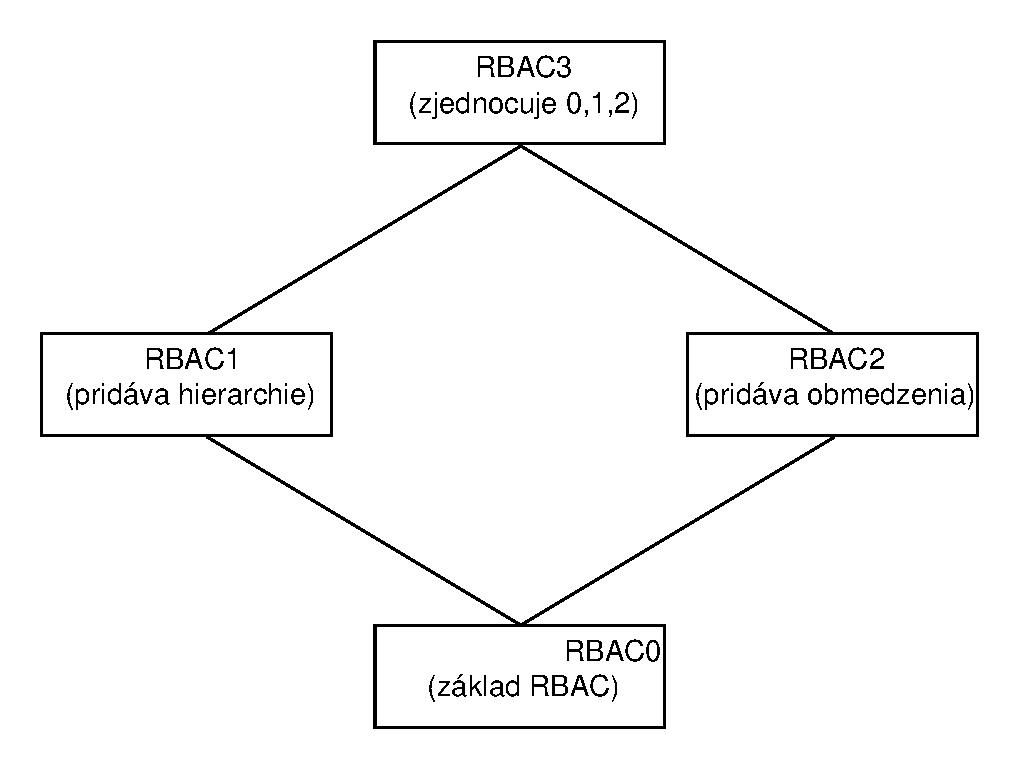
\includegraphics[width=0.7\textwidth]{images/rbac012}}
	\caption{Framework RBAC96 podľa Sandhu a spol.}
	\label{obr:roly_rbac0_rbac1_...}
\end{figure}



\subsubsection{Jadro RBAC}
Jadro RBAC , taktiež značené ako RBAC0 poskytuje základ pre riadenie prístupu na základe rol. Rozlišuje päť základných administratívnych prvkov: používateľov, roly a oprávnenia, pričom oprávnenia pozostávajú z operácii aplikovaných na objekty. Základ RBAC pozostáva z definovania oprávnení pre roly a používatelia sú priradení k roliam a tým nadobúdajú právomoci patriace rolám. Obrázok \ref{obr:rbac_kuhn} ukazuje vzťah užívateľov, rolí a oprávnení. Dvojitá šípka značí vzťah m:n. Teda napríklad jeden používateľ môže byť priradený k viacerým roliam a zároveň jedna rola môže pozostávať z mnohých používateľov. Tento princíp predstavuje flexibilné riešenie priradenia práv rolám a užívateľov k rolám, čím podporuje princíp minimálnych oprávnení. Každé oprávnenie predstavuje kombináciu objektov a operácii. Celý systém oprávnenia na základe môžeme vidieť na obrázku \ref{obr:rbac_kuhn_full}.

%users<->roles<->premissions
\begin{figure}[h]
	\centerline{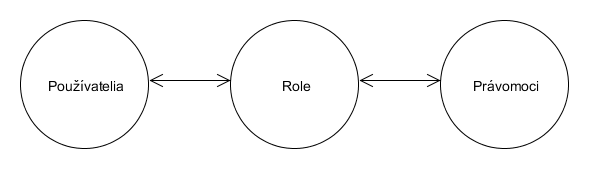
\includegraphics[width=0.7\textwidth]{images/rbac_kuhn}}
	\caption{Vzťahy RBAC podľa \cite{kuhn}}
	\label{obr:rbac_kuhn}
\end{figure}

%users<->roles<->(objescts, operations)
\begin{figure}[h]
	\centerline{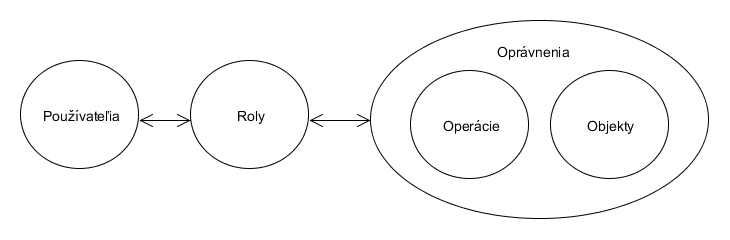
\includegraphics[width=0.7\textwidth]{images/rbac_kuhn_full}}
	\caption{Rozšírené vzťahy RBAC podľa \cite{kuhn}}
	\label{obr:rbac_kuhn_full}
\end{figure}



\subsubsection{Hierarchické štruktúry}
Mnoho rol v má v procesoch prelínajúce sa právomoci. Používatelia patriaci odlišným rolám môžu byť oprávnení vykonávať rovnaké operácie. Hierarchia rol zabezpečí prirodzené rozšírenie pre automatické splnomocňovanie nadradených rol. Môžeme si predstaviť napríklad juniorské a seniorské pozície v organizácii. Seniorská pozícia by mala mať obsahovať oprávnenia juniorskej, pričom môže zahŕňať oprávnenia, ktoré juniorskej pozícii neprináležia.   V opačnom smere to nie je možné.  Pre realizáciu hierarchickej štruktúry sa často zavádza relácia čiastočného usporiadania, ktorá verne znázorní štruktúru organizácie. 

%onkolog->doktor->sestrička
\begin{figure}[h]
	\centerline{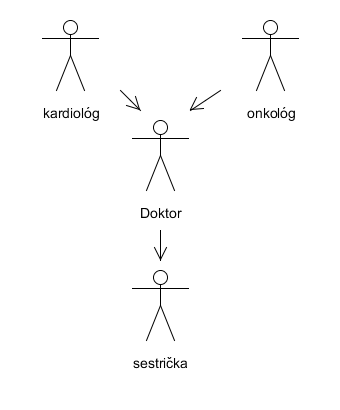
\includegraphics[height=0.45\textwidth]{images/hierarchia_priklad}}
	\caption{Príklad hierarchie rol}
	\label{obr:rbac_hierarchy}
\end{figure}






%(Telecom Glossary 2000, American National Standard for
%Telecommunications, American National Standards Institute)
\subsubsection{Obmedzenia}
Do modelu RBAC je možné pridať ďalšie obmedzenia, ktoré bližšie definujú politiku prístupu práv. Medzi tie základné patrí vylúčenie práv. V niektorých prípadoch chceme zamedziť aby používateľ mohol pristupovať súčasne k dvom objektom. \cite{telecom} definuje vylúčenie práv ako rozdelenie zodpovednosti pre citlivé údaje, tak aby žiaden jednotlivec nebol schopný narušiť bezpečnosť dát. Poznáme dve základné kategórie: statické a dynamické vylúčenie práv. Najľahšie ich rozlíšime podľa toho , v akom čase ich v systéme zavádzame. Statické vylúčenie práv sa určuje na začiatku a vopred zamedzí jednému používateľovi súčasne byť priradený v rolách, ktoré sa vzájomne vylučujú. Pri dynamickom vylúčení práv sa vylúčenie práv aplikuje v čase, keď je používateľ prihlásený v systéme. Tento typ vylúčenia je slabšou formou obmedzenia a dovoľuje jednému používateľovi zastávať dve vylučujúce sa role, avšak nemôže používať obidve v samotnej používateľskej session.



\subsection{Porovnanie RBAC s alternatívnymi metódami riadenia}
Okrem modelu RBAC existuje na trhu mnoho alternatívnych riešení riadenia prístupu. Zatiaľ čo RBAC rieši politiku prístupu na základe organizačnej štruktúry , ostatné metódy sa viac zameriavajú na bezpečnosť prístupu z pohľadu používateľa alebo administrátora. Zabezpečenie práv je definované až k používateľom.
V tejto časti si ukážeme tri časté modely: access control list (ACL), DAC (discretionary access control) a MAC (mandatory access control) .

	\begin{table}[h]%[17] R. Sandhu. Roles Versus Groups, 1996. http://www.list.gmu.edu/confrnc/rbac/rolegroup.	pdf
		\centering
		\begin{tabularx}{\textwidth}{>{\setlength\hsize{1\hsize}\setlength\linewidth{\hsize}}X>{\setlength\hsize{1\hsize}\setlength\linewidth{\hsize}}X>{\setlength\hsize{.7\hsize}\setlength\linewidth{\hsize}}X}
			RBAC & Štandartné systémy riadenia \\
			
			\begin{itemize}
				\item Rola nemusí obsahovať žiadnych používateľov
				\item Rola sa ľahko mapuje na štruktúru organizácie
				\item Prístupové práva sa mapujú na roly
				\item Používateľom sú priradené role
			\end{itemize}
			
			
			&
			
			\begin{itemize}
				\item Prístupové práva sú naviazané na používateľov 
				\item Používatelia sú rozdelení do skupín 
				\item Skupina je pomenovaná množina
				používateľov, práv a ďalších skupín,
				ktorá spravidla obsahuje aspoň dvoch
				používateľov
				\item Skupiny sa neviažu na štruktúru organizácie
			\end{itemize}
			
			
			
		\end{tabularx}
		\caption{Porovnanie RBAC so štandartými prístupmi riadenia}
		\label{tab:1}
	\end{table}


\subsubsection{ACL}
Tento prístup definuje ku každému objektu zoznam používateľov a ich právomocí. Administrátor v systéme ľahko vyhľadá kto má k akému objektu aké právomoci. Problém nastáva , ak chceme zistiť všetky právomoci , ktoré prináležia konkrétnemu používateľovi. Ešte väčšie komplikácie nastávajú pri potrebe upraviť alebo vymazať používateľovi nejaké právomoci, pretože treba prejsť všetky možné objekty v danom systéme. 


% [1] DoD, Trusted Computer System Evaluation Criteria (TCSEC), DoD 5200.28-STD.

\subsubsection{voliteľné riadenie prístupu DAC}
Podľa \cite{} DAC predstavuje riadenie prístupu k objektu založené na identite subjektu, skupiny alebo ich kombinácie. Subjekt, ktorý vlastní určité práva je schopný ich predávať  ďalšiemu subjektu. DAC teda necháva jednotlivým používateľom možnosť prideľovať a odoberať prístupové práva. Tento prístup však môže byť často nežiadúci, ak chceme zamedziť šíreniu dát medzi neoprávnených používateľov. DAC bližšie nešpecifikuje právomoci pre konkrétneho používateľa. Akonáhle môže používateľ k objektom pristupovať, môže dáta zmeniť alebo rozšíriť práva pre neautorizovaného používateľa.(Sandhu and Samarati, 1994)


% CURPHEY, Mark. Mandatory Access Control [online]. 2002 [cit. 2008-10-22] .
%Dostupné z WWW: <http://www.cgisecurity.com/owasp/html/ch08s02.html>
\subsubsection{povinné riadenie prístupu MAC}
Ako riešenie pre hlavný problém DAC architektúry, povinné riadenie prístupu MAC definuje hierarchické úrovne bezpečnosti. Vychyľuje sa tak od štandartných prístupov a implementuje MLS (multilevel security).  Iba administrátori sú oprávnení  spravovať a priraďovať prístupové práva. Ku každému objektu ako aj subjektu sa priradí určitá bezpečnostnú úroveň. Riadenie prístupu je následne automaticky riadené pomocou dvoch pravidiel. Prvé z nich povoľuje  čítať v rovnakej a nižšej bezpečnostnej úrovni, zatiaľ čo druhé zabezpečuje zapisovanie do rovnakej alebo vyššej bezpečnostnej úrovne. 

 % MAC (Mandatory access control) predstavuje tyký typ riadenia, v ktorom môžu iba administrátori spravovať a priraďovať prístupové práva. Nad každým objektom administrátor definuje politiku prístupu pre každý subjekt samostatne. 


\subsection{Výhody RBAC}
V podnikovej oblasti prináša RBAC model revolúciu pre riadenie prístupu. Tento systém výrazne zjednodušuje administratívu, čo v konečnom dôsledku zvyšuje celkovú produktivitu a znižuje náklady.  Všeobecne platí, že čím viac používateľov sa v systéme vyskytuje, tým je výhodnejšie a efektívnejšie použiť tento systém. Systém RBAC sa ukazuje ako atraktívna náhrada alternatívnych modelov. V \cite{ekonomika} NIST popísala ekonomickú návratnosť zavedenia RBAC do systému. Môžeme vidieť (obr. \ref{obr:rbac_net_cash}), že návratnosť investície rastie s časom používanie. Hlavné výhody RBAC sú

\begin{itemize}
	\item rýchla administrácia - najťažšie pri systéme RBAC je definovať na začiatku jej štruktúru. Neskôr pri pridávaní nových užívateľov nie je zväčša potrebné vytvárať novú rolu, ale iba priradiť nového používateľa do už existujúcich rol. Pri zmene alebo odstránení používateľa z firmy nevznikajú problémy s odstraňovaním a mazaním právomocí
	\item zrozumiteľnosť - zväčša sa na definovanie rol používajú termíny blízke človeku ako lekár, manažér, programátor. Takéto riadenie práv je teda pre človeka prirodzenejšie ako ostatné zaužívané metódy. Ľudia tak nevynaložia veľa úsilia na samotné študovanie administrácie rol. 
	\item nové možnosti bezpečnosti - statické a dynamické vylúčenie práv
\end{itemize} 

%net cash
\begin{figure}[h]
	\centerline{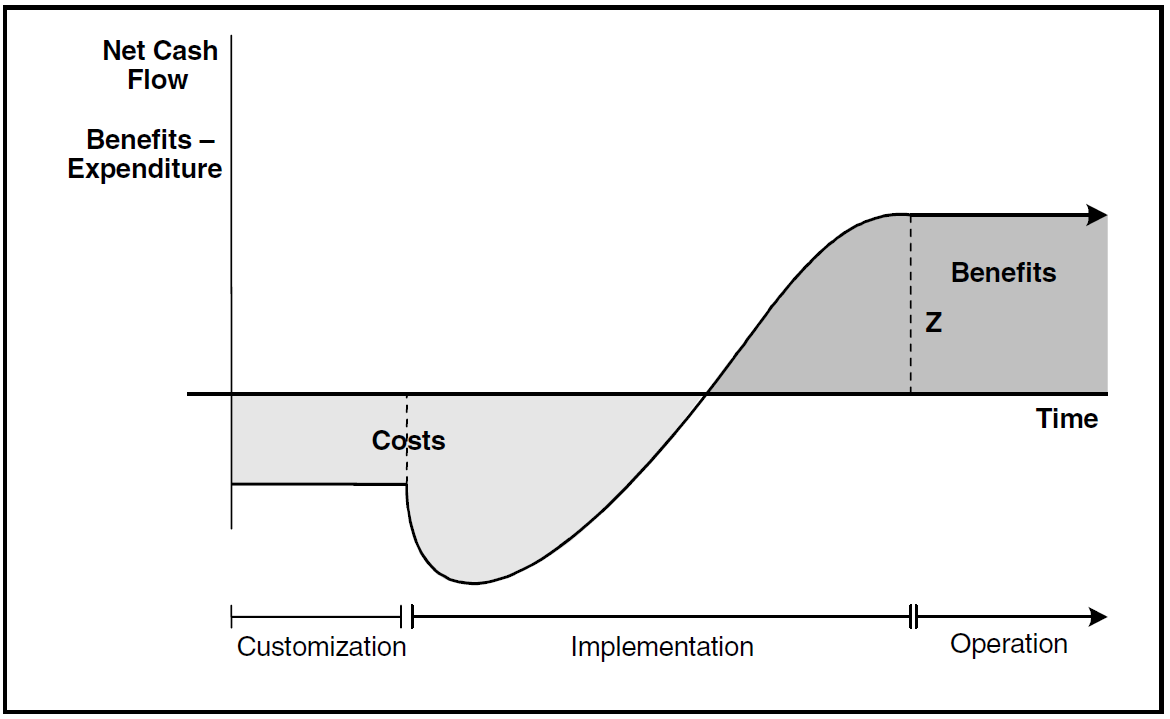
\includegraphics[width=0.6\textwidth]{images/rbac_net_cash}}
	\caption{Ekonomická návratnosť RBAC podľa \cite{ekonomika}}
	\label{obr:rbac_net_cash}
\end{figure}


%---------------------------------- Koniec sekcie RBAC ----------------------------------------










	


